\documentclass[t]{beamer}
\title{Building Recommender Systems}
\subtitle{Lecture 7}
\author{Boris Shminke}
\institute{Université Côte d'Azur, CNRS, LJAD, France}
\date{03/01/2021}
\AtBeginSection[]{
  \begin{frame}
    \frametitle{Outline}
    \tableofcontents[currentsection]
  \end{frame}
}
\begin{document}
\begin{frame}
  \titlepage  
\end{frame}  
\begin{frame}
  \frametitle{Outline}
  \tableofcontents
\end{frame}
\section{Introduction}
\begin{frame}
  \frametitle{What is cold-start?}
  \begin{itemize}
  \item collaborative filtering works better than content based
  \item but it demands a user having long enough history
  \item what to recommend to new users (with a few or no interactions)?
  \item how to recommend new or less known items?
  \end{itemize}
\end{frame}
\section{Cold Start in Neighbourhood-based Recommendations}
\begin{frame}
  \frametitle{Neighbourhood-based Recommender}
  $$\hat{r}_{ui}=\sum\limits_jS_{ij}r_{uj}$$

  where

  $r_{uj}$ --- (observed) rating of item $j$ given by user $u$

  $S_{ij}$ --- a similarity measure between items $i$ and $j$

  $\hat{r}_{ui}$ --- (predicted) rating of item $i$ given by user $u$
\end{frame}  
\begin{frame}
  \frametitle{Collaborative Neighbourhood-based Recommender}
  \begin{itemize}
  \item $\hat{r}_{ui}=\sum\limits_jS_{ij}r_{uj}$
  \item $S_{ij}$ is based on user interactions
  \item if $i$ is a new item, $S_{ij}=0$
  \end{itemize}
\end{frame}
\begin{frame}
  \frametitle{Content-based Neighbourhood-based Recommender}
  \begin{itemize}
  \item $\hat{r}_{ui}=\sum\limits_jS_{ij}r_{uj}$
  \item $S_{ij}$ is based on item features only
  \item if $i$ is a new item, still sometimes $S_{ij}\ne0$
  \end{itemize}
\end{frame}
\begin{frame}
  \frametitle{Hybrid Neighbourhood-based Recommender}
  \begin{itemize}
  \item $\hat{r}_{ui}=\alpha\sum\limits_jA_{ij}r_{uj}+\left(1-\alpha\right)\sum\limits_jB_{ij}r_{uj}$
  \item $A_{ij}$ is based on user interactions
  \item $B_{ij}$ is based on item features
  \item no cold-start problem!
  \end{itemize}
\end{frame}
\begin{frame}
  \frametitle{Hybrid Neighbourhood-based Recommender}
  \begin{itemize}
  \item $\hat{r}_{ui}=\alpha\sum\limits_jA_{ij}r_{uj}+\left(1-\alpha\right)\sum\limits_jB_{ij}r_{uj}$
  \item $\alpha$ can depend on the number of users who rated item $i$
  \item for example, $\alpha$ can be zero if item collected more than 10 ratings from different users
  \end{itemize}
\end{frame}
\begin{frame}
  \frametitle{Hybrid Neighbourhood-based Recommender}
  \begin{itemize}
  \item $\hat{r}_{ui}=\alpha\sum\limits_jA_{ij}r_{uj}+\left(1-\alpha\right)\sum\limits_jB_{ij}r_{uj}$
  \item no cold-start problem for items!
  \item still can't recommend anything to new users
  \end{itemize}
\end{frame}
\begin{frame}
  \frametitle{Universal Recommender} $$\hat{r}_{ui}=\alpha_1\sum\limits_jA_{1,ij}r_{1,uj}+\alpha_2\sum\limits_jA_{2,ij}r_{2,uj}+\dots+\alpha_n\sum\limits_jA_{n,ij}r_{n,uj}$$

  where

$\hat{r}_{ui}$ --- (predicted) probability of user $u$ making a target action with item $i$

$A_{1,ij},A_{2,ij},\dots$ --- a matrices of co-occurrences of actions of type $1,2,\dots$ on item $j$ with the target action on item $i$.

$r_{1,uj},r_{2,uj},\dots$ --- histories of actions of type $1,2,\dots$ for user $u$

$\alpha_1,\alpha_2,\dots$ --- model hyper-parameters, balancing different types of actions
\end{frame}
\begin{frame}
  \frametitle{Universal Recommender} $$\hat{r}_{ui}=\alpha_1\sum\limits_jA_{1,ij}r_{1,uj}+\alpha_2\sum\limits_jA_{2,ij}r_{2,uj}+\dots+\alpha_n\sum\limits_jA_{n,ij}r_{n,uj}$$
\begin{itemize}
\item uses a variety of interactions: buy, add to basket, add to wishlist, recommend to a friend, comment, like, report, abandon\dots
\item can recommend items with no target interactions
\item can recommend to users who have no target interactions
\end{itemize}
\end{frame}
\begin{frame}
  \frametitle{Universal Recommender} $$\hat{r}_{ui}=\alpha_1\sum\limits_jA_{1,ij}r_{1,uj}+\alpha_2\sum\limits_jA_{2,ij}r_{2,uj}+\dots+\alpha_n\sum\limits_jA_{n,ij}r_{n,uj}$$
\begin{itemize}
\item popularized by \href{https://actionml.com/}{ActionML} in 2015
\item open-sourced as \href{https://attic.apache.org/projects/predictionio.html}{PredictionIO} (in Apache Attic since Sep 2020)
\item uses very basic, but very powerful idea
\end{itemize}
\end{frame}
\begin{frame}
  \frametitle{Cold Start in Neighbourhood-based Recommendations} \begin{itemize}
\item easy to implement and scalable
\item can use item features (for cold items)
\item can use non-target actions (for cold users and items)
\end{itemize}
\end{frame}
\section{Cold Start in Latent Factors Recommendations}
\begin{frame}
  \frametitle{Latent Factors Recommendations}
  $$\hat{r}_{ui}=\left<x_u,y_i\right>$$

  where

  $\hat{r}_{ui}$ --- (predicted) rating of item $i$ given by user $u$
  
  $x_u$ --- latent representation (embedding) of a user $u$
  
  $y_i$ --- latent representation (embedding) of a user $i$
  
  $\left<.,.\right>$ --- inner product
\end{frame}  
\begin{frame}
  \frametitle{Latent Factors Recommendations}
  $$\hat{r}_{ui}=\left<x_u,y_i\right>$$
  \begin{itemize}
  \item $x_u$ and $y_i$ can be results of matrix decomposition
  \item $x_u$ and $y_i$ are learn as embedding layers in a deep neural network
  \end{itemize}
\end{frame}  
\begin{frame}
  \frametitle{Latent Factors Recommendations}
  $$\hat{r}_{ui}=\left<x_u,y_i\right>$$
  \begin{itemize}
  \item if user is new, $x_u$ is unknown, can't recommend
  \item if item is new, $y_i$ is unknown, can't recommend
  \item true for users and items not known at training time
  \item training a very resource intense (MF and especially DL)  
  \end{itemize}
\end{frame}  
\begin{frame}
  \frametitle{Similarity-based Solution}
  $$\hat{y_i}=\sum\limits_jS_{ij}y_j$$

  where
  
  \begin{itemize}
  \item $\hat{y_i}$ --- predicted embedding for a new item $i$
  \item $y_j$ --- embeddings of known items, similar to $i$
  \item $S_{ij}$ --- (pre-processed) similarity measure between items $i$ (new) and $j$ (known ones)
  \end{itemize}
\end{frame}  
\begin{frame}
  \frametitle{Deep Learning Solution: CB2CF}
  \begin{itemize}
  \item $\hat{y_i}$ is defined as a NN from item features
  \item the model is trained on known items and their embeddings
  \item \href{https://dl.acm.org/doi/10.1145/3298689.3347038}{published} by Microsoft in 2019  
  \end{itemize}
\end{frame}  
\begin{frame}
  \frametitle{CB2CF: Content-to-Collaborative filtering}
  \begin{enumerate}
  \item train a NN on know items and users interaction
  \item train two more NNs for features-to-embedding maps for users and items
  \item for new items and users get embeddings from features
  \item get recommendations from embeddings  
  \end{enumerate}
\end{frame}  
\begin{frame}
  \frametitle{CB2CF: Content-to-Collaborative filtering}
  \begin{figure}
    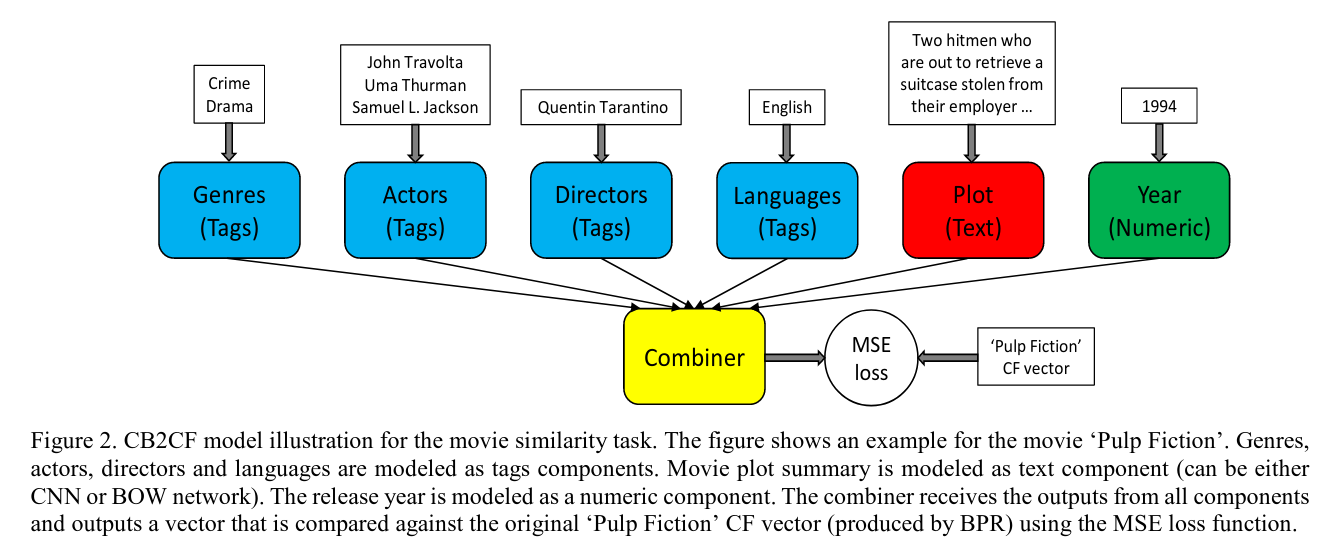
\includegraphics[scale=0.25]{CB2CF}
  \end{figure}
  RecSys '19: Proceedings of the 13th ACM Conference on Recommender SystemsSeptember 2019 Pages 228–236

  https://doi.org/10.1145/3298689.3347038
\end{frame}
\begin{frame}
  \frametitle{CB2CF: Content-to-Collaborative filtering}
  \begin{itemize}
  \item relatively simple solution
  \item works well with both new items and new users
  \item requires training several models instead of one  
  \end{itemize}
\end{frame}
\section{Folding In}
\begin{frame}
  \frametitle{Embeddings for New Items in Real-Time}
  \begin{itemize}
  \item getting embeddings usually requires (re)training the model
  \item model training is always done separatly from serving (inference)
  \item model training is resource intense, expensive, and slow process  
  \end{itemize}
\end{frame}
\begin{frame}
  \frametitle{Embeddings for New Items in Real-Time}
  \begin{itemize}
  \item if a user had no history during model training we can't easily get their embedding even if after model training the user accumulated history
  \item no user embedding means no recommendations
  \item but why not to recommend to a user who already has history?
  \end{itemize}
\end{frame}
\begin{frame}
  \frametitle{Folding In}
  $$\sum\limits_{u,i}\left(\left<x_u,y_i\right>-r_{ui}\right)^2\longrightarrow\min_{x_u,y_i}$$
  \begin{itemize}
  \item a well known loss function
  \item can be minimized using ALS (as matrix factorization)
  \item can be minimized using SGD (as a neural network)
  \end{itemize}  
\end{frame}
\begin{frame}
  \frametitle{Folding In}
  $$\sum\limits_i\left(\left<x',y_i\right>-r_{u'i}\right)^2+\sum\limits_{u,i}\left(\left<x_u,y_i\right>-r_{ui}\right)^2\longrightarrow\min_{x',x_u,y_i}$$
  \begin{itemize}
  \item suppose we already found the minimum
  \item now we add new $r_{u'i}$ for a previously unknown user $u'$
  \end{itemize}  
\end{frame}
\begin{frame}
  \frametitle{Folding In}
  $$\sum\limits_i\left(\left<x',y_i\right>-r_{u'i}\right)^2\longrightarrow\min_{x'}$$
  \begin{itemize}
  \item we can minimize for new ratings of a new user separately
  \item we also assume that several interactions of one user won't affect previously found embeddings of items $y_i$
  \item we arrive at linear regression of dimension $N$ (embedding dimension)
  \end{itemize}  
\end{frame}
\begin{frame}
  \frametitle{Folding In}
  $$\sum\limits_i\left(\left<x',y_i\right>-r_{u'i}\right)^2\longrightarrow\min_{x'}$$
  \begin{itemize}
  \item very simple technique to embed new users in real time
  \item works both for matrix factorization (e.g. ALS or SVD)
  \item also can work for neural networks (e.g. with doing optimization steps for couple SGD batches with new data)
  \end{itemize}
\end{frame}
\section{Rating Elicitation}
\begin{frame}
  \frametitle{Possible New User Scenario}
  \begin{itemize}
  \item a new website or app, many new users
  \item no information about new users coming to our app
  \item we can buy some information but that's impractical
  \item users don't want to share information about them
  \end{itemize}
\end{frame}
\begin{frame}
  \frametitle{Rating Elicitation}
  \begin{itemize}
  \item we ask users which items they interacted before
  \item or which items they liked (not in our app)
  \item or which items they would like to see in our app
  \item we use those ratings instead of real interactions
  \end{itemize}
\end{frame}
\begin{frame}
  \frametitle{Rating Elicitation: Problem}
  \begin{itemize}
  \item we ask users which items they interacted before
  \item we need to show several to choose
  \item those items should be popular
  \item and also they should be diverse
  \end{itemize}
\end{frame}
\begin{frame}
  \frametitle{Popularity and Diversity of Embeddings}
  \begin{itemize}
  \item the more popular item is, the larger the embedding norm
  \item the more unsimilar items are, the larger the angle between the embeddings
  \item (that works for inner-product based models!)
  \end{itemize}
\end{frame}
\begin{frame}
  \frametitle{Popularity and Diversity of Embeddings}
\begin{figure}
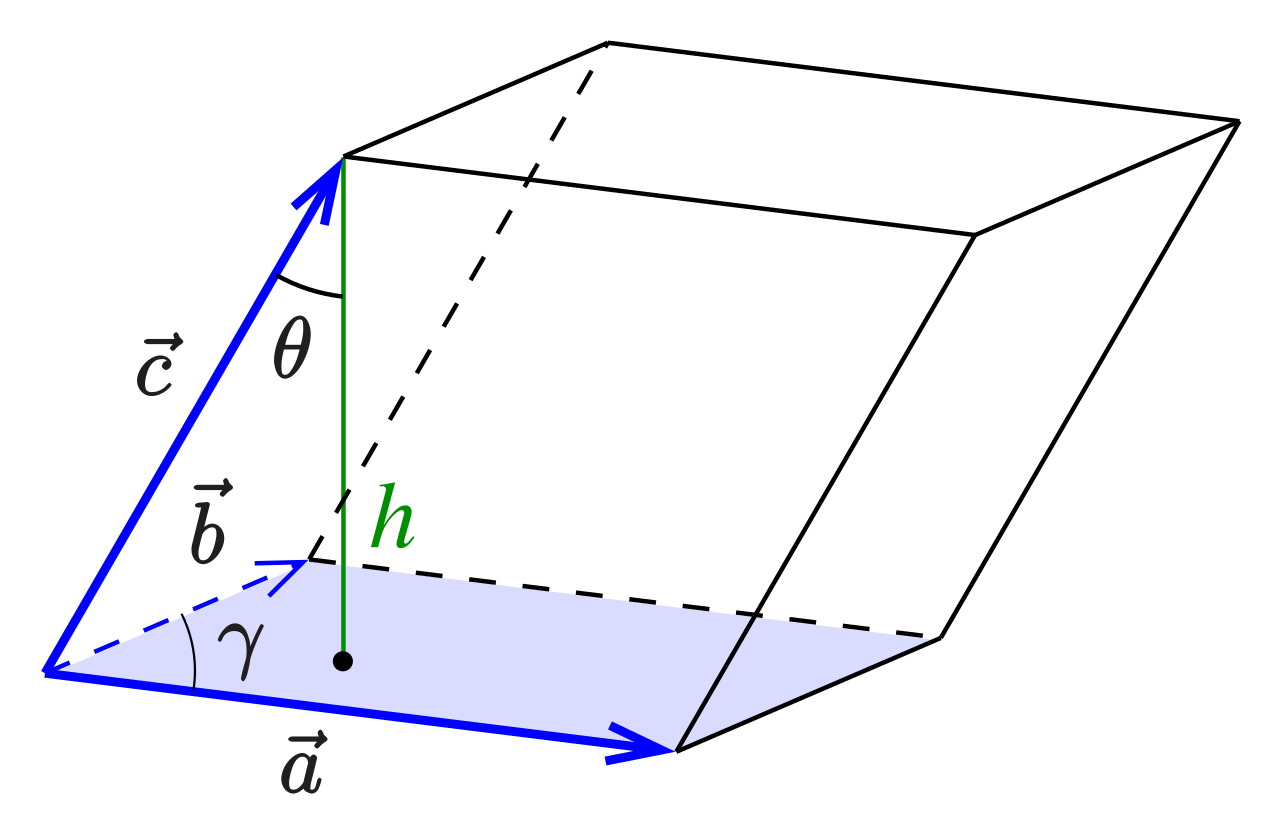
\includegraphics[scale=0.2]{parallelepiped}
\end{figure}
\end{frame}
\begin{frame}
  \frametitle{Popularity and Diversity of Embeddings}
  \begin{itemize}
  \item embeddings can form a parallelepiped of some volume
  \item the larger the embedding norm, the greater the volume
  \item the larger the angle between the embeddings, the greater the volume
  \item ergo: we need to maximize volume!
  \end{itemize}
\end{frame}
\begin{frame}
  \frametitle{Generalized Volume}
  \begin{itemize}
  \item volume in $N$-dimensional embedding space is defined only for $N$ vectors (edges of the parallelepiped)
  \item if we want to choose $M\ne N$ vectors, what to maximize?
  \item $\det A$ is a volume of a parallelepiped formed by vectors $A_i$ (columns of the matrix $A$)
  \item generalized volume is defined as $\det A^TA$
  \end{itemize}
\end{frame}
\begin{frame}
  \frametitle{Generalized Volume}
  \begin{itemize}
  \item generalized volume is defined as $\det A^TA$
  \item $\det A^TA=\prod\limits_{i=1}^N\sigma_i$ where $\sigma_i$ are singular values of matrix $A$
  \item generalized volume maximization problem is related to SVD  
  \end{itemize}
\end{frame}
\begin{frame}
  \frametitle{Maximal Generalized Volume}
  \begin{itemize}
  \item generalized volume is defined as $\det A^TA$
  \item generalized volume maximization problem is related to SVD
  \item there is a Python package \href{https://pypi.org/project/maxvolpy/}{\texttt{maxvolpy}} for computing it
  \end{itemize}
\end{frame}
\begin{frame}
  \frametitle{Rating Elicitation with MaxVol}
  \begin{itemize}
  \item build a recommender (get embeddings of items)
  \item apply rectangular MaxVol on embeddings
  \item show user the suggested subset of items
  \item recommend for the new user as if they had history (e.g. using folding in)
  \end{itemize}
\end{frame}
\end{document}
